\documentclass[12pt,letterpaper]{article}
\usepackage{datetime} %maybe don't need
\usepackage{amsmath}
\usepackage{amsfonts}
\usepackage{amssymb}
\usepackage{graphicx}
\usepackage{natbib}
\usepackage{url}
\usepackage{setspace}
\usepackage{geometry}

%I added the following
\usepackage[colorlinks=true, linkcolor=black, citecolor=black, urlcolor=black]{hyperref} %for text hyperlinks
\usepackage{graphicx}
\usepackage{longtable} %for Gerstmann
\usepackage{booktabs}  %for pretty tables
\usepackage{lscape} %forget where horizontal comes from
\usepackage{rotating} %forget where horizontal comes from
\usepackage{tabularx}  %to help format tables

% Adjust margins to fit the AER style
\geometry{top=1in, bottom=1in, left=1in, right=1in}

% Title setup
\title{Implications of the Federal Legalization of Same-Sex Marriage on Interstate Migration in the US}
\author{Noah Rich\footnote{University of Michigan, njrich@umich.edu.}}
\date{\today}

% Start the document
\begin{document}

\maketitle
\footnote{Acknowledgements:}

% Abstract section
\begin{abstract}
    tbd
\end{abstract}

\newpage

% Main content section
\section{Introduction}

tbd

\section{Literature Review}
Over the past 30 years, the legal landscape for individuals in same-sex relationships has changed dramatically in the United States. In 1996, Congress passed the Defense of Marriage Act (DOMA), which defined marriage as being strictly between a man and a woman \citep{5}. Seven short years later, Massachusetts became the first state to legalize same-sex marriage \citep{1, 3, 5}. Between then and 2015, more than half of all U.S. states followed \citep{12}. In 2013, the Supreme Court invalidated DOMA’s definition of marriage, and in 2015, legalized same-sex marriage outright \citep{1, 3, 5, 12}. This incredible period of flux has brought many questions: how might those in same-sex and opposite-sex relationships respond differently to marriage access? Might this impact interstate migration? Many researchers have attempted to answer these questions, at least in part.

Economists have been interested in marriage since at least the 1970s. In a landmark series of papers, \citet{9} described how marriage can be understood in a traditional cost-benefit choice utility framework. Specifically, two people enter a marriage if, and only if, it increases both of their lifetime utility \citep{9}. Many unique benefits can be ascribed to marriage in the US. Legally, there are at least 1,138 benefits listed in federal law, including rights related to citizenship, taxes, benefits, healthcare, and parenthood \citep{1, 8}. Non-legal benefits include social status and a concrete symbol of commitment \citep{8}. On the other hand, costs include legal fees, and partner searching and marriage consideration costs \citep{9}. As marriage can then be understood as a good with costs and benefits, it can be understood as something that many people might pay to obtain. 

These people, notably, include both those who would want to marry someone of the same or opposite sex. However, as stated above, individuals in same-sex relationships could not marry anywhere in the US until 2003 \citep{1, 3, 5, 12}. This follows a general trend defining the differences between those in same-sex and opposite-sex relationships: while there might be many similarities between those in same-sex and opposite sex relationships: outside social and legal factors, unrelated to sexuality, often determine differences \citep{2}. Researchers have noted these differences in education level, relationship structure, income, likelihood to have children, and importantly, living location \citep{2, 11, 6, 7, 8, 10, 7}. Gay men and lesbian women tend to be more highly educated than heterosexual people \citep{2, 7, 11}. Same-sex cohabiting relationships tend to form at a lower rate than opposite-sex cohabiting relationships; however, same-sex relationships tend to be less homogenous across age and racial lines \citep{2, 7}. Gay men tend to earn less than straight men, while lesbian women tend to earn more than straight women \citep{6}. Those in same-sex relationships face higher costs to raising children, and tend to have children at lower rates than those in opposite sex relationships \citep{8, 10, 11}. Finally, gay men and lesbian women tend to live in different places than their heterosexual counterparts: gay men, similar to straight men without children, often choose to live in expensive, high-amenity places like San Francisco \citep{7, 10, 11, 13}. Again crucially, this follows the pattern described above by (2): sexuality might play some role in this difference, but another factor- likelihood to have children- can also plays a role.

Understanding this, that many of these differences might not be attributable purely to sexuality but other outside factors, researchers have studied how marriage legalization differences on a statewide basis impacted those in same-sex relationships relative to those in opposite-sex relationships. Overall, researchers have found some convergence in outcomes between those in same-sex and opposite-sex relationships in states where same-sex marriage was legalized. \citep{3} found some evidence that the legalization of same-sex marriage led to the better integration of those in same-sex relationships into the labor market and thus higher employment. With the tax, health insurance, and adoption rights allowed by legal marriage, same-sex spouses began to specialize more in paid work or unpaid housework and childcare \citep{3, 4, 6}. Further, legal same-sex marriage brought a degree of social acceptance: there is some evidence that same-sex marriage legalization led to more popular support for same-sex marriage \citep{3, 21}. When more outside factors were similar, individuals in same-sex and opposite-sex relationships began to share more similarities.

Above, I discuss ways same-sex marriage increased similarities between those in same-sex and opposite-sex relationships. However, there are areas where it would make sense that state-by-state legalization might bring more differences. Namely, interstate migration. Below, I discuss how economists understand migration, and how it connects to same-sex marriage legalization.

Economists also understand migration in a traditional cost-benefit framework \citep{12, 8}. When the utility of a different state is greater than the utility of one’s current state and costs of moving, an individual might want to move to a new state. Monetary costs and benefits include state-related income differences and moving costs \citep{1, 15, 16, 17}. Non-monetary costs and benefits might include distance from family, place attachment, and general satisfaction \citep{1, 15}. Crucially, individuals in same-sex relationships might have also considered the legal status of same-sex marriage before 2015. As these costs and benefits vary across different people with different preferences, this model then predicts different migration decisions for different people. Younger and more educated people- those potentially less place-attached- might be more likely to move \citep{17}. Those in a household with other family members- all attached to each other yet all with non-identical preferences- might be less likely to move \citep{16}. It is important to note, however, that none of these groups are monoliths, which can have significant implications for their migration outcomes \citep{20}. 

In addition to age, education, and family, researchers have studied the migration impacts of same-sex marriage legalization for those in same-sex relationships. Using an events study empirical framework, \citet{1} found that states with legal same-sex marriage pulled individuals in same-sex relationships. Using a probit model, \cite{12} found that states without legal same-sex marriage pushed out household heads in same-sex relationships. This follows the logic that individuals in same-sex relationship would see same-sex marriage as a factor in migration decisions in a way that individuals in opposite-sex relationships would not. There is an endogeneity concern that other factors that impact same-sex marriage legalization also impact same-sex migration, but these can be controlled for using state and time fixed effects \citep{5}. 

After 2015, same-sex marriage ceased to be a differentiating factor between states for individuals in same-sex relationships. Like how same-sex marriage conveyed a certain level of convergence between same-sex and opposite-sex individuals within legalized states, federal same-sex marriage could convey a certain level of convergence for state-by-state migration. Unlike the questions discussed above, this has not been studied as extensively. This is what the rest of this paper will be about. 




\section{Model}
\subsection{Theoretical Framework}
Following \citet{1, 12, 18}, I state that an individual moves from their current state to another state when the utility of moving is positive, does not move when the utility of moving is negative, and is indifferent when the utility of moving is zero. In this framework, the utility of moving is a function of the utility to individual i of the possible new state n, the utility to individual i of the current state c, and moving costs m. Utilities of a given place are themselves functions of the characteristics of a given place and the characteristics of individual i. This can be seen in the following equation: 

\begin{equation}
U(\text{moving to place}_i) = U(\text{new place}_i) - U(\text{current place}) - C(\text{moving})
\end{equation}

\begin{equation}
U(\text{place}_i \text{ for person}_j) = F(\text{characteristics of person}_j, \text{characteristics of place}_i)
\end{equation}


In between 2003 and 2015, I argue that for same-sex individuals, legalized same-sex marriage is a relevant state characteristic when making migration decisions. For opposite-sex individuals, I argue that it isn’t. This is because in this period, opposite-sex individuals had access to marriage in all states, while same-sex individuals only had access to marriage in some states. This would make same-sex marriage a differentiator for same-sex individuals, if not opposite-sex individuals. As marriage conveys numerous benefits, same-sex individuals should see access to marriage as a benefit, and lack of marriage as a cost. It is also important to note that locally legalized same-sex marriage might convey other benefits for same-sex individuals, such as social acceptance \citep{12}. However, I argue that after 2015, this difference for same-sex and opposite-sex people should begin to decrease. Under Obergefell v Hodges, marriage is equally accessible across the US for same-sex individuals, just as for opposite-sex people. 

\subsection{Empirical Framework}

To test this theory, I use a triple differences specification \citep{23, 24, 25}. This model exploits my prediction that I expect same-sex marriage to affect same-sex individuals but not opposite-sex individuals, different states that locally legalized same-sex marriage did so at different times, and that Obergefell v Hodges impacted every state in the US at the same time. To get at any asymmetric effects of locally legalized same-sex marriage as a pull factor to a state or as a push factor from a state, I run two parallel specifications. They are as follows:

%<pull eqn>
In-Migration:
\begin{equation}
\text{migrate}_{i,t} = \alpha \cdot (\text{interactions})_{i,t} 
+ \beta \cdot (\text{samesex} \times \text{post2015} \times \text{locally legalized})_{i,t} 
+ \text{FE}_{i,t} + X_{i,t} + \epsilon_{i,t}
\end{equation}

Out-Migration:
\begin{equation}
\text{migrate}_{i,t} = 
\alpha \cdot (\text{interactions})_{i,t,t-1} + \beta \cdot (\text{samesex} \times \text{post2015} \times \text{locally legalized})_{i,t,t-1} + \text{FE}_{i,t,t-1} + X_{i,t} + \epsilon_{i,t}
\end{equation}

In both, the outcome variable is if individual i migrated from state c to a different state state n in year t. In both, the main interaction term crosses a dummy variable for whether individual i is same-sex or not, whether year t is past 2015 or not, and whether the state of interest has locally legalized same-sex marriage or not in year t. In the pull model, the state of interest is the state individual i is in at time t. In the push model, the state of interest is the state individual i is in at time t - 1. In both, (FE) refers to time and state fixed effects for the state of interest. This captures any state and time-specific factors that might impact same-sex migration, such as state population, income, and attitude differences across states and time. (X) is a vector of controls, which depending on specification can include sex, race, education, age, income, parenthood, and birth state. Designed to support the parallel trends assumptions needed in a triple difference specification, these follow similar controls used in similar studies by citep{1, 3, 5, 7, 12}. Frequency weights are used.

In both models, the coefficient of interest is (beta). When (beta) is negative in the pull model, that can be interpreted as there being a decrease in same-sex people moving to locally legalized states after 2015 relative to opposite-sex people. When (beta) is zero in the pull model, that can be interpreted as there being no change in the amount of same-sex people moving to locally legalized states after 2015 relative to opposite-sex people. When (beta) is positive in the pull model, that can be interpreted as there being an increase in the amount of same-sex people moving to locally legalized states after 2015 relative to opposite-sex people. When (beta) is negative in the push model, that can be interpreted as there being a decrease in same-sex people moving from locally legalized states after 2015 relative to opposite-sex people. When $\beta$ is zero in the push model, that can be interpreted as there being no change in the amount of same-sex people moving from locally legalized states after 2015 relative to opposite-sex people. When $\beta$ is positive in the push model, that can be interpreted as there being an increase in the amount of same-sex people moving from locally legalized states after 2015 relative to opposite-sex people. I would expect $\beta$ to be symmetrically negative in the pull model and positive in the push model.

To further isolate any relationships, I run heterogeneity tests across age groups and state legalization type. While all the individuals in my sample are in relationships, they are not all of the same age nor from states of the same legalization type. Individuals of different ages have different propensities to move, meaning that same-sex legalization could have differences across age groups \citep{1, 17}.  I expect opposite results for individuals originating from states locally legalized and not, so it can be helpful to run separate regressions on each group.

The code and data I use can be found here: https://github.com/nj-rich/same-sex-migration. This excludes the raw Census data I downloaded from IPUMS.

\section{Data}

The main dataset used in this paper covers all 50 U.S. states and Washington D.C. in the period 2011 − 2019. It comes from the American Community Survey (ACS) compiled in the Integrated Public Use Microdata Series (28). The ACS is an annual nationwide survey with observations at the individual level. The only other data I use includes the years that same-sex marriage was announced as legalized in each state. This comes from (27). Massachusetts was the first state to legalize same-sex marriage in 2003; by 2015, 37 total states had legal same-sex marriage.

\begin{longtable}{|c|c|}
\hline
\textbf{State} & \textbf{Year of Same-Sex Marriage Legalization} \\
\hline
Massachusetts & 2003 \\
Connecticut & 2008 \\
Iowa & 2009 \\
New Hampshire & 2009 \\
District of Columbia & 2009 \\
Vermont & 2009 \\
New York & 2011 \\
Maine & 2012 \\
Maryland & 2012 \\
Washington & 2012 \\
California & 2013 \\
Delaware & 2013 \\
Hawaii & 2013 \\
Illinois & 2013 \\
Minnesota & 2013 \\
New Jersey & 2013 \\
New Mexico & 2013 \\
Rhode Island & 2013 \\
Alaska & 2014 \\
Arizona & 2014 \\
Colorado & 2014 \\
Idaho & 2014 \\
Indiana & 2014 \\
Kansas & 2014 \\
Montana & 2014 \\
Nevada & 2014 \\
North Carolina & 2014 \\
Oklahoma & 2014 \\
Oregon & 2014 \\
Pennsylvania & 2014 \\
South Carolina & 2014 \\
Utah & 2014 \\
Virginia & 2014 \\
West Virginia & 2014 \\
Wisconsin & 2014 \\
Wyoming & 2014 \\
Alabama & 2015 \\
Arkansas & 2015 \\
Florida & 2015 \\
Georgia & 2015 \\
Kentucky & 2015 \\
Louisiana & 2015 \\
Michigan & 2015 \\
Mississippi & 2015 \\
Missouri & 2015 \\
Nebraska & 2015 \\
North Dakota & 2015 \\
Ohio & 2015 \\
South Dakota & 2015 \\
Tennessee & 2015 \\
Texas & 2015 \\
\hline
\end{longtable}
\textbf{Note: }This table shows the year in which same-sex marriage was \textit{most recently} legalized in each state as recorded by \citet{1}.


The ACS dataset allows for the indirect identification of an individual’s relationship type and migration status. The (27) dataset allows for the identification of a state’s same-sex marriage legalization status. The ACS records if an individual is in a relationship with someone that lives in their household, and if they are, whether their partner has their same gender or not. This enables the identification of individuals in same-sex and opposite-sex relationships. It is important to note that this means individuals in same-sex or opposite-sex relationships with partners that live in a different household will be classified as partnerless. Further, this means I do not directly identify individuals who identify as homosexual or heterosexual. However, this is the highest level of detail afforded in this survey. Ultimately, this comes out to about 1 percent of survey respondents per year (28). The ACS also records an individual’s current state of residence and which state they lived in the year prior. This allows for the direct identification of interstate migrants. In both the push and pull model, I attribute a state’s legalization status to the current year, not the prior year. I justify this on the grounds that this promotes consistency and it is not always clear if an individual’s move occurred in the prior or current year. I determine whether a state locally legalized same-sex marriage or not by whether in a current year they have legal same-sex marriage, and if they do, if the legalization occurred before the Supreme Court legalized same-sex marriage at the federal level in 2015. About 67 percent percent of the country lived in locally-legalized states in 2014. 

\begin{table}[htbp]

\caption{Summary Statistics for Overall Population}
\label{tab:overall_table}
\centering
\begin{tabular}[t]{rrrr}
\toprule
\multicolumn{2}{c}{ } & \multicolumn{2}{c}{\% in \textit{Obergefell}-legalized States} \\
\cmidrule(l{3pt}r{3pt}){3-4}
Year & \% Same-Sex & Same-Sex & Different-Sex\\
\midrule
2011 & 1 & 90 & 86\\
2012 & 1 & 85 & 80\\
2013 & 1 & 67 & 57\\
2014 & 1 & 37 & 31\\
2015 & 1 & 37 & 32\\
\addlinespace
2016 & 2 & 37 & 32\\
2017 & 2 & 37 & 33\\
2018 & 2 & 37 & 33\\
2019 & 2 & 37 & 34\\
\bottomrule
\end{tabular}
\end{table}


To better isolate the relationships I care about, I impose a series of restrictions on the ACS sample. While the ACS includes information on residents of US territories and US residents who did not live in a US state in the prior year, I exclude those from my sample. I do this to restrict my sample to regions for which I have data on legal same-sex marriage and to all potential inter-state migrants. Someone who moves from Argentina to Colorado can never qualify as an interstate mover. I also restrict my sample to those identified as being in a same-sex or opposite-sex relationship. (1, 16) have noted that those in relationships often behave differently than those not in relationships, meaning this restriction allows for more plausible comparison across groups. Finally, I exclude individuals born out of the US. One of the controls I include in my empirical specification is birth state, with the understanding that if someone lives in a state that is not their birth state they are more likely to move back to their birth state (12). This control will affect those not born in a US state differently than those born in a US state in the context of my inter-state migration model, justifying the exclusion of those non-US born.

I also apply several restrictions for technical reasons. I exclude observations in which the ACS has identified errors in coding an individual’s sex or has identified an individual’s sex as missing. While researchers have noted that ACS more reliably identifies individuals in same-sex relationships after 2012, other researchers have noted that before this there were sex-coding reliability issues before this (3, 5, 7, 12). Dropping these observations ensures more reliable identification of individuals in same-sex relationships. I also drop observations with missing age, education, and race information and unknown employment status and income status. I do this because all of these variables are used as controls in my model.

\begin{landscape}
\tiny
\begin{table}

\caption{Summary Statistics for Proposed Controls}
\centering
\begin{tabular}[t]{rrrrrrrrrrr}
\toprule
\multicolumn{1}{c}{ } & \multicolumn{2}{c}{Fraction Female} & \multicolumn{2}{c}{Mean Age} & \multicolumn{2}{c}{Fraction At Least 4 Years College} & \multicolumn{2}{c}{Fraction White} & \multicolumn{2}{c}{Mean Income} \\
\cmidrule(l{3pt}r{3pt}){2-3} \cmidrule(l{3pt}r{3pt}){4-5} \cmidrule(l{3pt}r{3pt}){6-7} \cmidrule(l{3pt}r{3pt}){8-9} \cmidrule(l{3pt}r{3pt}){10-11}
Year & Same-Sex & Opposite-Sex & Same-Sex & Opposite-Sex & Same-Sex & Opposite-Sex & Same-Sex & Opposite-Sex & Same-Sex & Opposite-Sex\\
\midrule
2011 & 0.496 & 0.500 & 49.422 & 46.054 & 0.315 & 0.412 & 0.813 & 0.798 & 42767.20 & 47310.34\\
2012 & 0.496 & 0.501 & 49.635 & 46.146 & 0.323 & 0.421 & 0.811 & 0.811 & 44091.95 & 49406.49\\
2013 & 0.495 & 0.499 & 49.809 & 46.975 & 0.327 & 0.413 & 0.807 & 0.804 & 45632.95 & 50450.91\\
2014 & 0.496 & 0.502 & 50.005 & 46.886 & 0.334 & 0.415 & 0.804 & 0.792 & 46754.82 & 52758.57\\
2015 & 0.496 & 0.507 & 50.178 & 46.789 & 0.341 & 0.425 & 0.801 & 0.796 & 48733.81 & 53395.28\\
\addlinespace
2016 & 0.497 & 0.491 & 50.410 & 46.799 & 0.349 & 0.435 & 0.797 & 0.780 & 50181.30 & 55306.73\\
2017 & 0.497 & 0.507 & 50.565 & 46.609 & 0.358 & 0.433 & 0.794 & 0.779 & 51792.06 & 56273.47\\
2018 & 0.497 & 0.499 & 50.689 & 46.305 & 0.363 & 0.440 & 0.791 & 0.771 & 53819.73 & 57059.85\\
2019 & 0.498 & 0.509 & 50.894 & 44.921 & 0.370 & 0.447 & 0.789 & 0.764 & 56634.86 & 58998.77\\
\bottomrule
\end{tabular}
\end{table}

\end{landscape}

In further robustness checks and heterogeneity analyses, I restrict the sample further in different ways. These are discussed in other sections. 

\clearpage

\section{Results}


\subsection{Main Model}
\clearpage
\begin{figure}
    \centering
    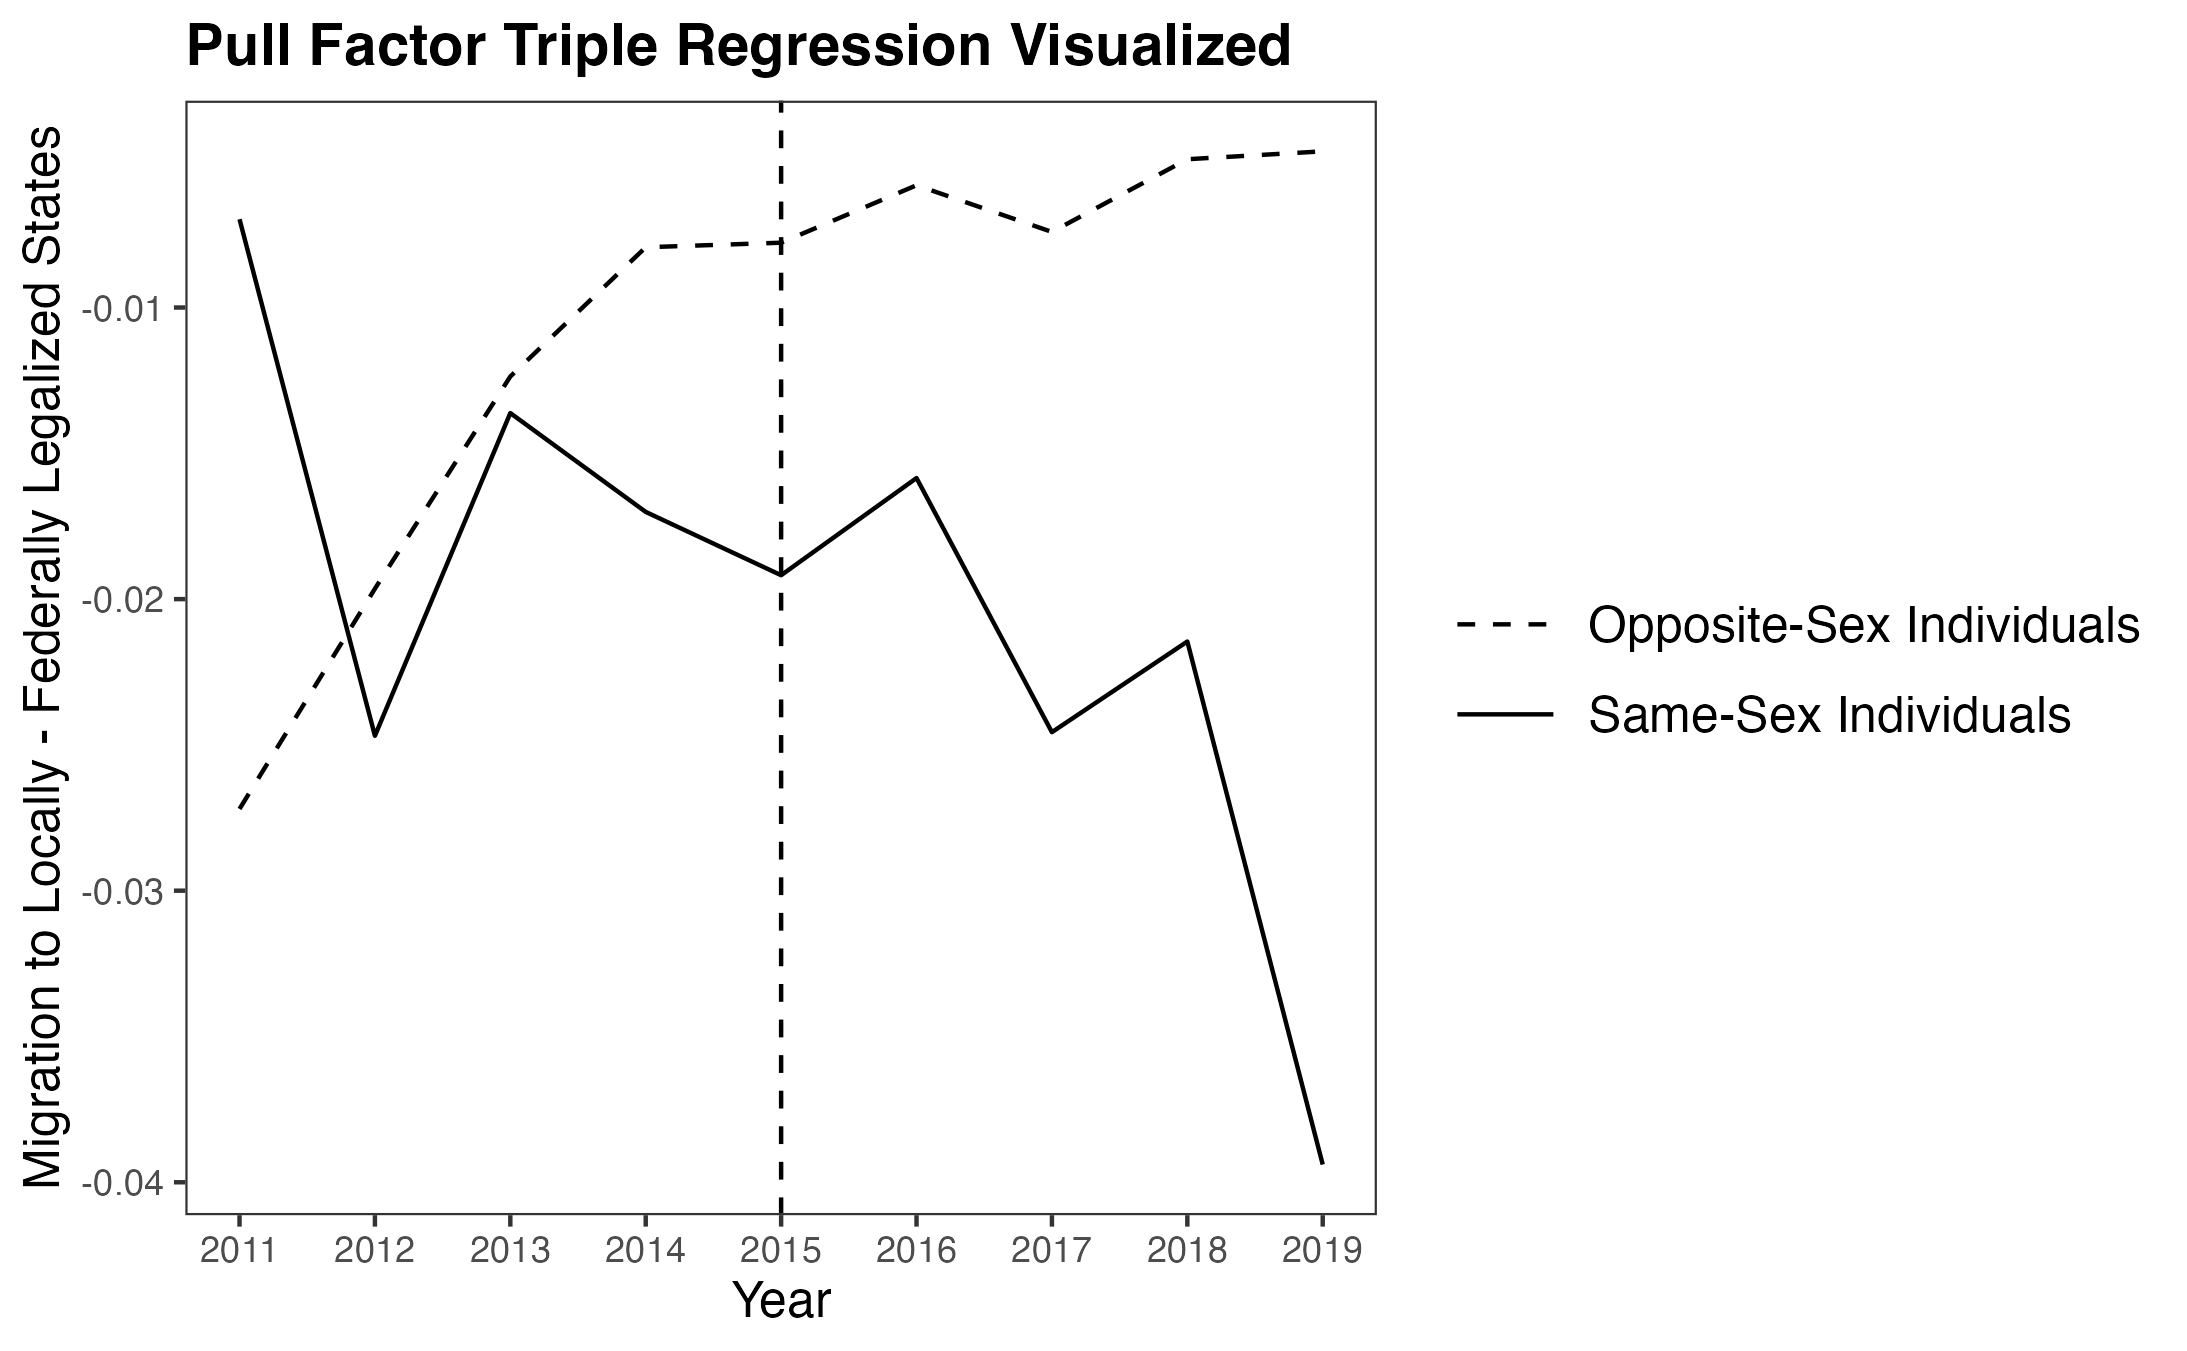
\includegraphics[width=1\linewidth]{outputs/summary_stats/post_diffs.png}
    \label{fig:enter-label}
\end{figure}

\begin{tabular}{lccc}
\multicolumn{4}{c}{Ex-Post Model} \\ \hline
 & (1) & (2) & (3) \\
VARIABLES & migrant & migrant & migrant \\ \hline
 &  &  &  \\
1.in\_samesex\#1.expost\_old\_legal\#1.post\_2015 & -0.015* & -0.013* & 0.013 \\
 & (0.007) & (0.006) & (0.033) \\
Constant & 0.106*** & 0.394*** & 3.356*** \\
 & (0.001) & (0.008) & (0.080) \\
 &  &  &  \\
Observations & 956,236,912 & 956,236,912 & 956,236,912 \\
 R-squared & 0.004 & 0.070 & 0.921 \\ \hline
\multicolumn{4}{c}{ Robust standard errors in parentheses} \\
\multicolumn{4}{c}{ *** p$<$0.01, ** p$<$0.05, * p$<$0.1} \\
\multicolumn{4}{c}{ Model 1 includes interaction terms and fixed effects only.} \\
\multicolumn{4}{c}{ )} \\
\multicolumn{4}{c}{ )} \\
\multicolumn{4}{c}{ )} \\
\multicolumn{4}{c}{ )} \\
\end{tabular}


\begin{figure}
    \centering
    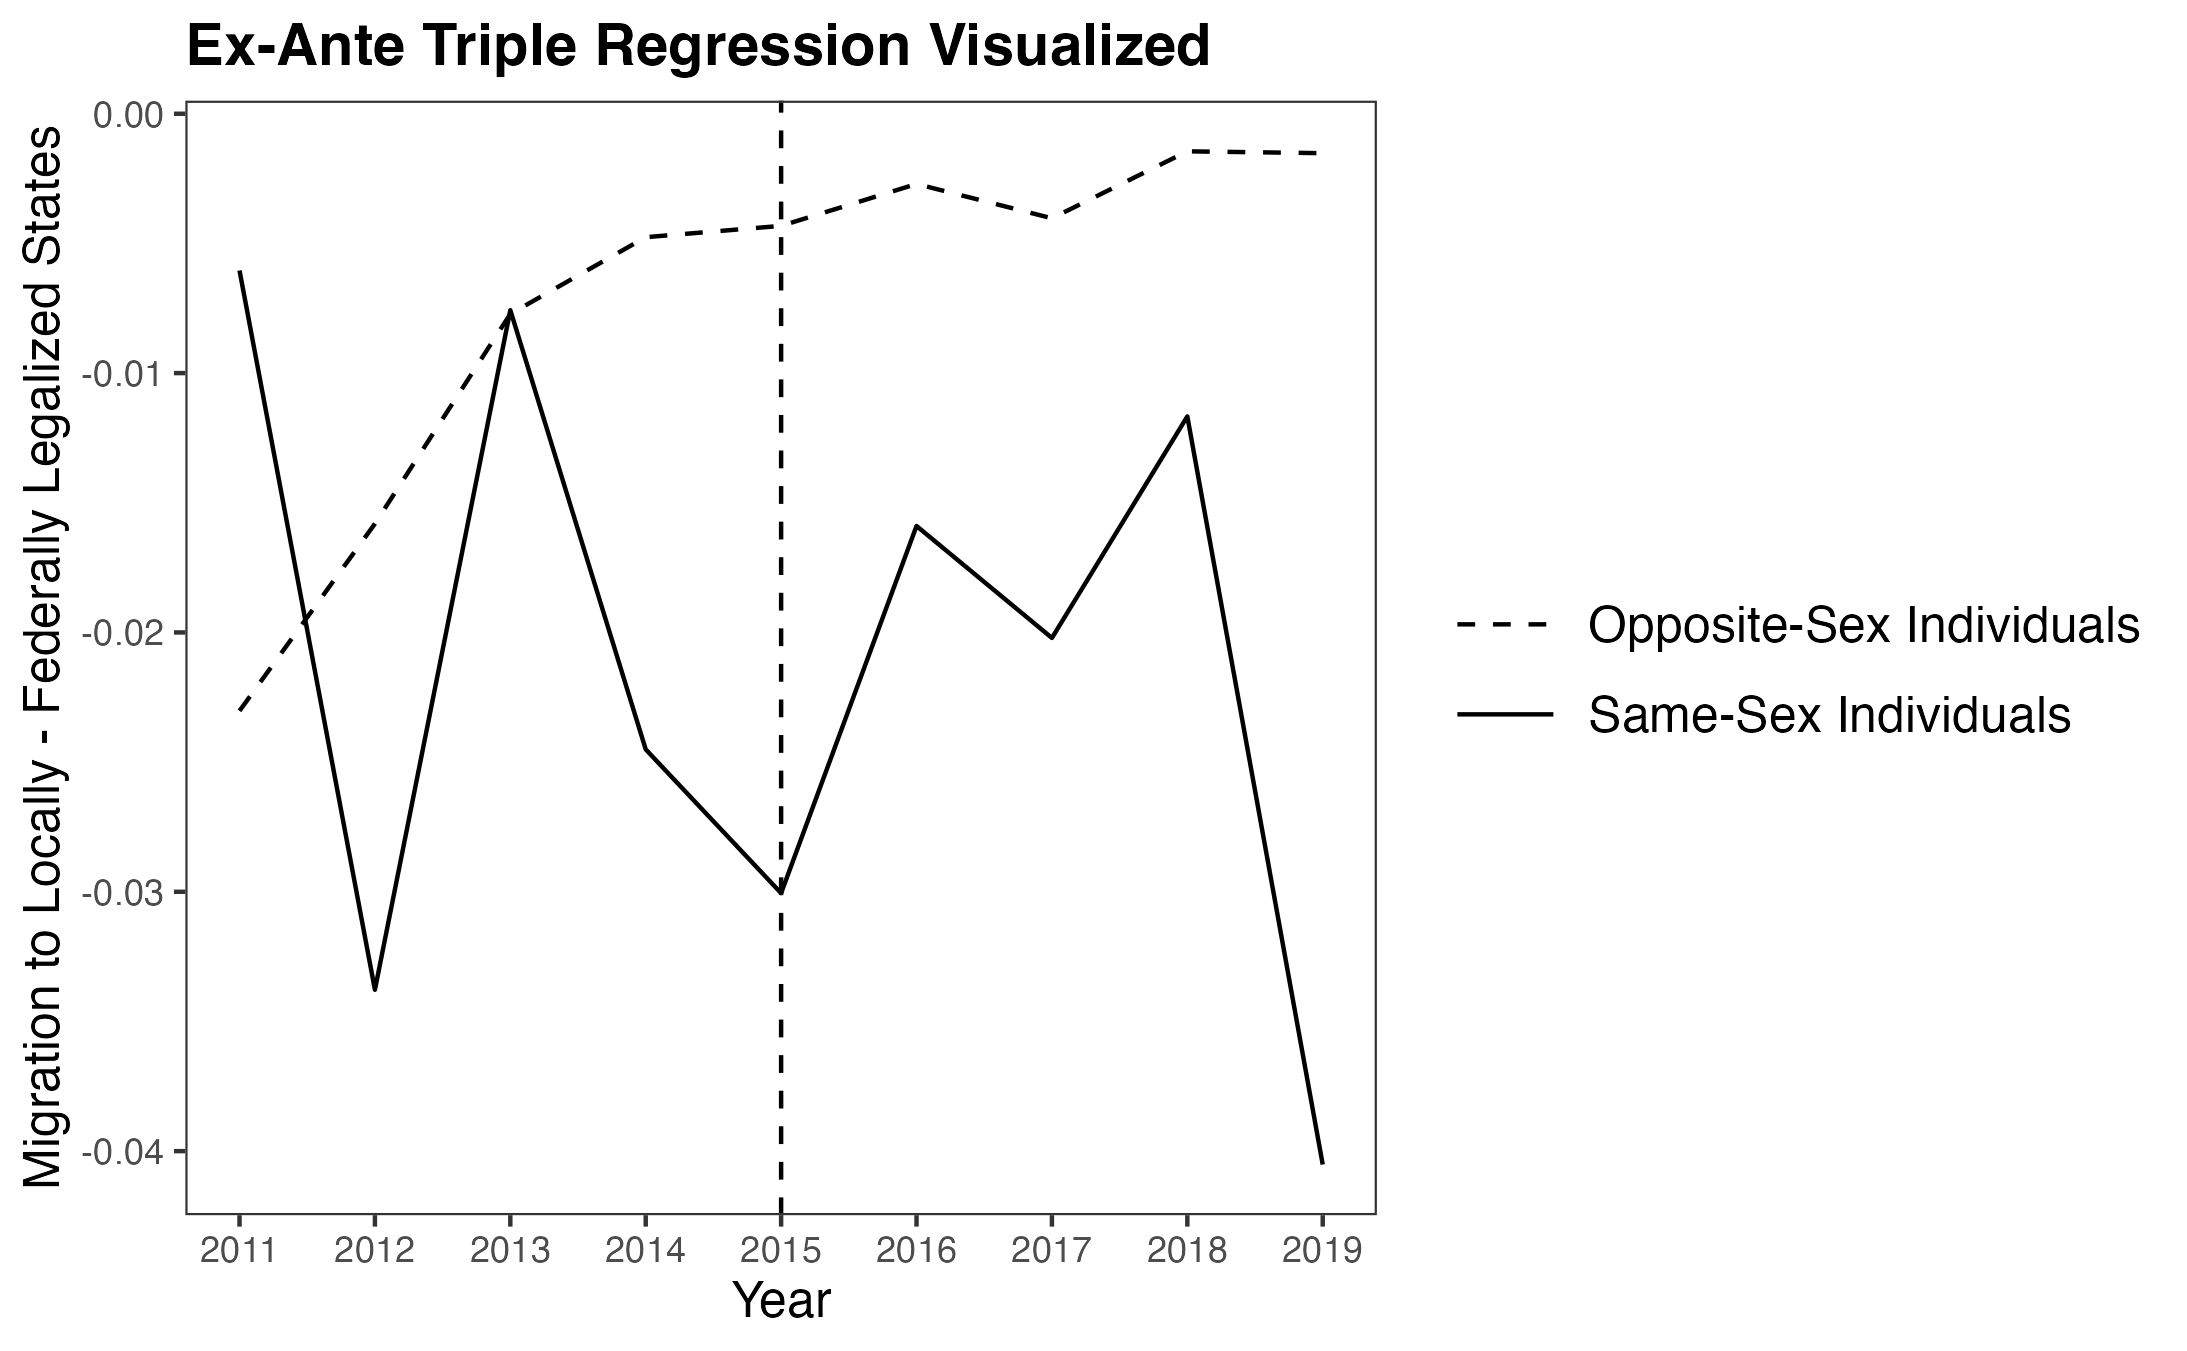
\includegraphics[width=1\linewidth]{outputs/summary_stats/ante_diffs.png}
    \label{fig:enter-label}
\end{figure}

\begin{tabular}{lccc}
\multicolumn{4}{c}{Ex-Ante Model} \\ \hline
 & (1) & (2) & (3) \\
VARIABLES & migrant & migrant & migrant \\ \hline
 &  &  &  \\
1.in\_samesex\#1.exante\_old\_legal\#1.post\_2015 & -0.016 & -0.014 & 0.014 \\
 & (0.009) & (0.008) & (0.030) \\
Constant & 0.106*** & 0.394*** & 3.757*** \\
 & (0.001) & (0.007) & (0.123) \\
 &  &  &  \\
Observations & 956,236,912 & 956,236,912 & 956,236,912 \\
 R-squared & 0.003 & 0.069 & 0.912 \\ \hline
\multicolumn{4}{c}{ Robust standard errors in parentheses} \\
\multicolumn{4}{c}{ *** p$<$0.01, ** p$<$0.05, * p$<$0.1} \\
\multicolumn{4}{c}{p{\textwidth}}{ Model 1 includes interaction terms and fixed effects only. \newline
Model 2 includes interaction terms, fixed effects, and controls for sex, race, education, age, and income. \newline
Model 3 includes interaction terms, fixed effects, and controls for sex, race, education, age, income, and birthstate. \newline
Models 1 and 2 use a weighted sample. Model 3 uses a weighted and collapsed sample.} \\
\multicolumn{4}{c}{ )} \\
\multicolumn{4}{c}{ )} \\
\multicolumn{4}{c}{ )} \\
\multicolumn{4}{c}{ )} \\
\end{tabular}


%subsubsections for flow directions?

\subsection{Heterogeneity Test: Gender Split Sample}
\clearpage

\begin{figure}
    \centering
    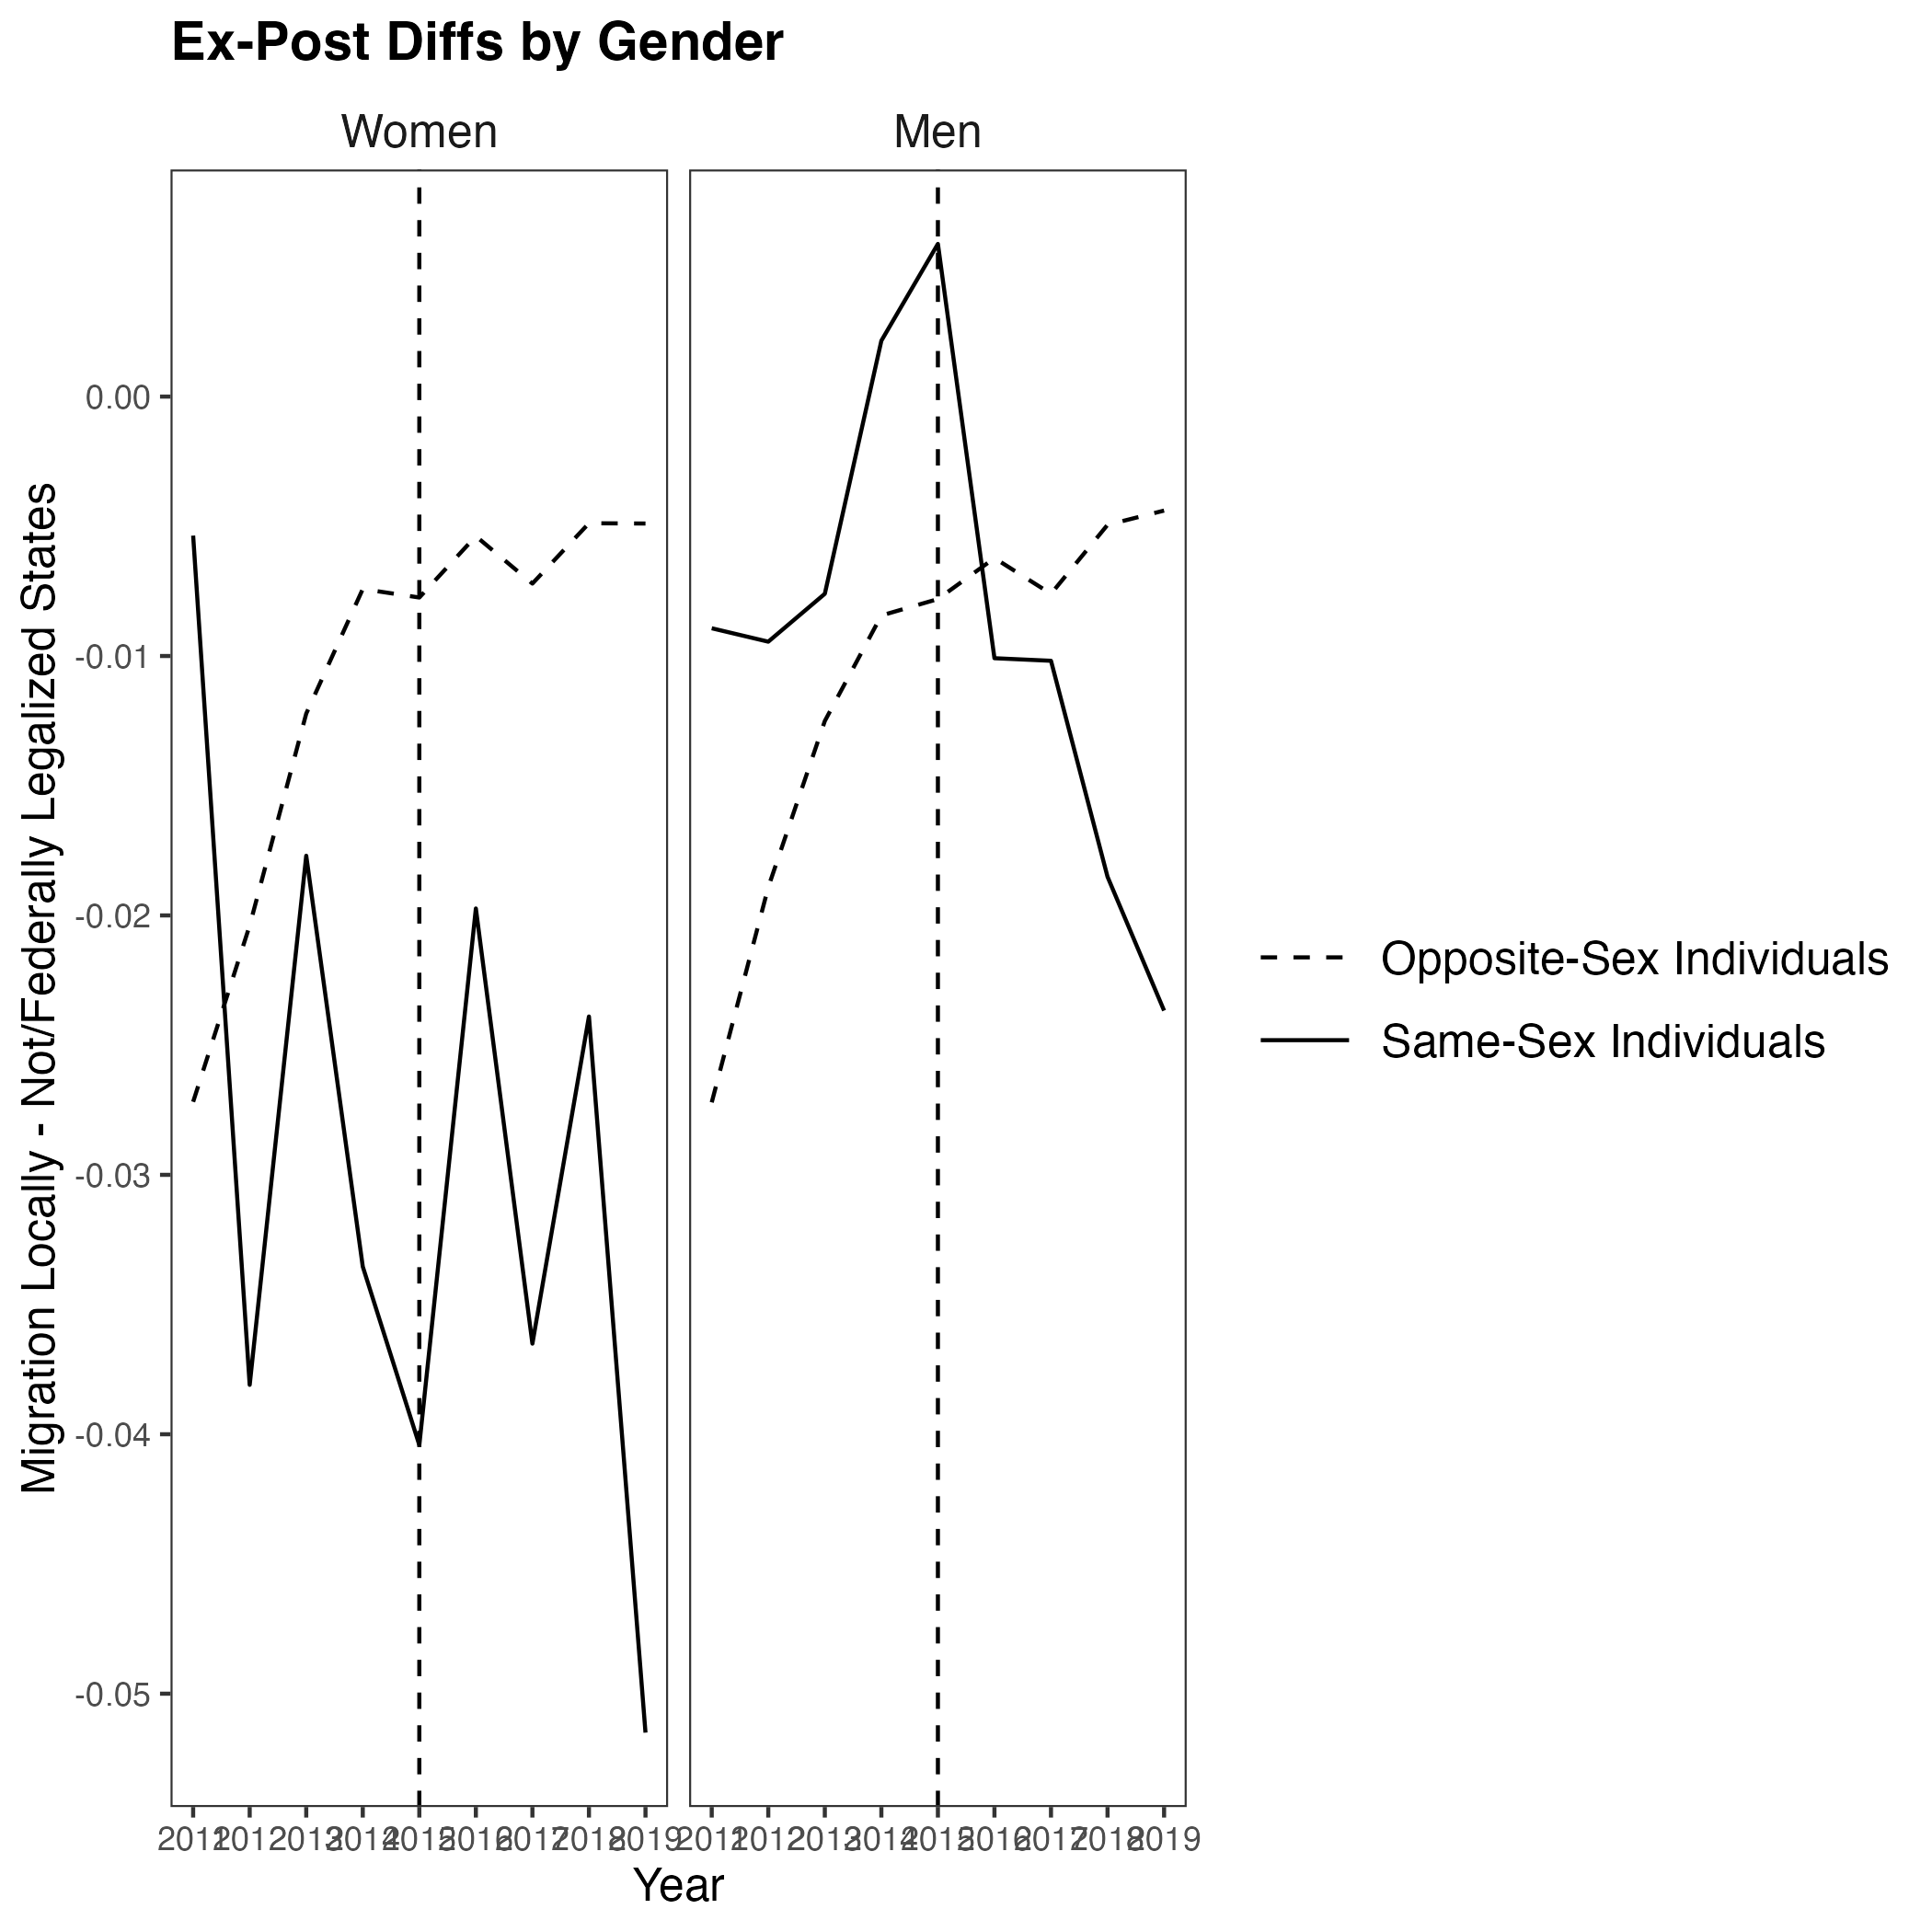
\includegraphics[width=1\linewidth]{outputs/summary_stats/sex_post_diffs.png}
    \label{fig:enter-label}
\end{figure}

%\begin{landscape}
\centering
\tiny
\begin{tabular}{lc}
\multicolumn{2}{c}{Ex-Post Model by Sex} \\ \hline
 & (1) \\
VARIABLES & Model 1: Men \\ \hline
 &  \\
1.in\_samesex\#1.expost\_old\_legal\#1.post\_2015 & -0.005*** \\
 & (0.001) \\
Constant & 0.106*** \\
 & (0.001) \\
 &  \\
Observations & 481,915,892 \\
 R-squared & 0.004 \\ \hline
\multicolumn{2}{c}{ Robust standard errors in parentheses} \\
\multicolumn{2}{c}{ *** p$<$0.01, ** p$<$0.05, * p$<$0.1} \\
\multicolumn{2}{c}{ See below.} \\
\end{tabular}

%\end{landscape}

\begin{figure}
    \centering
    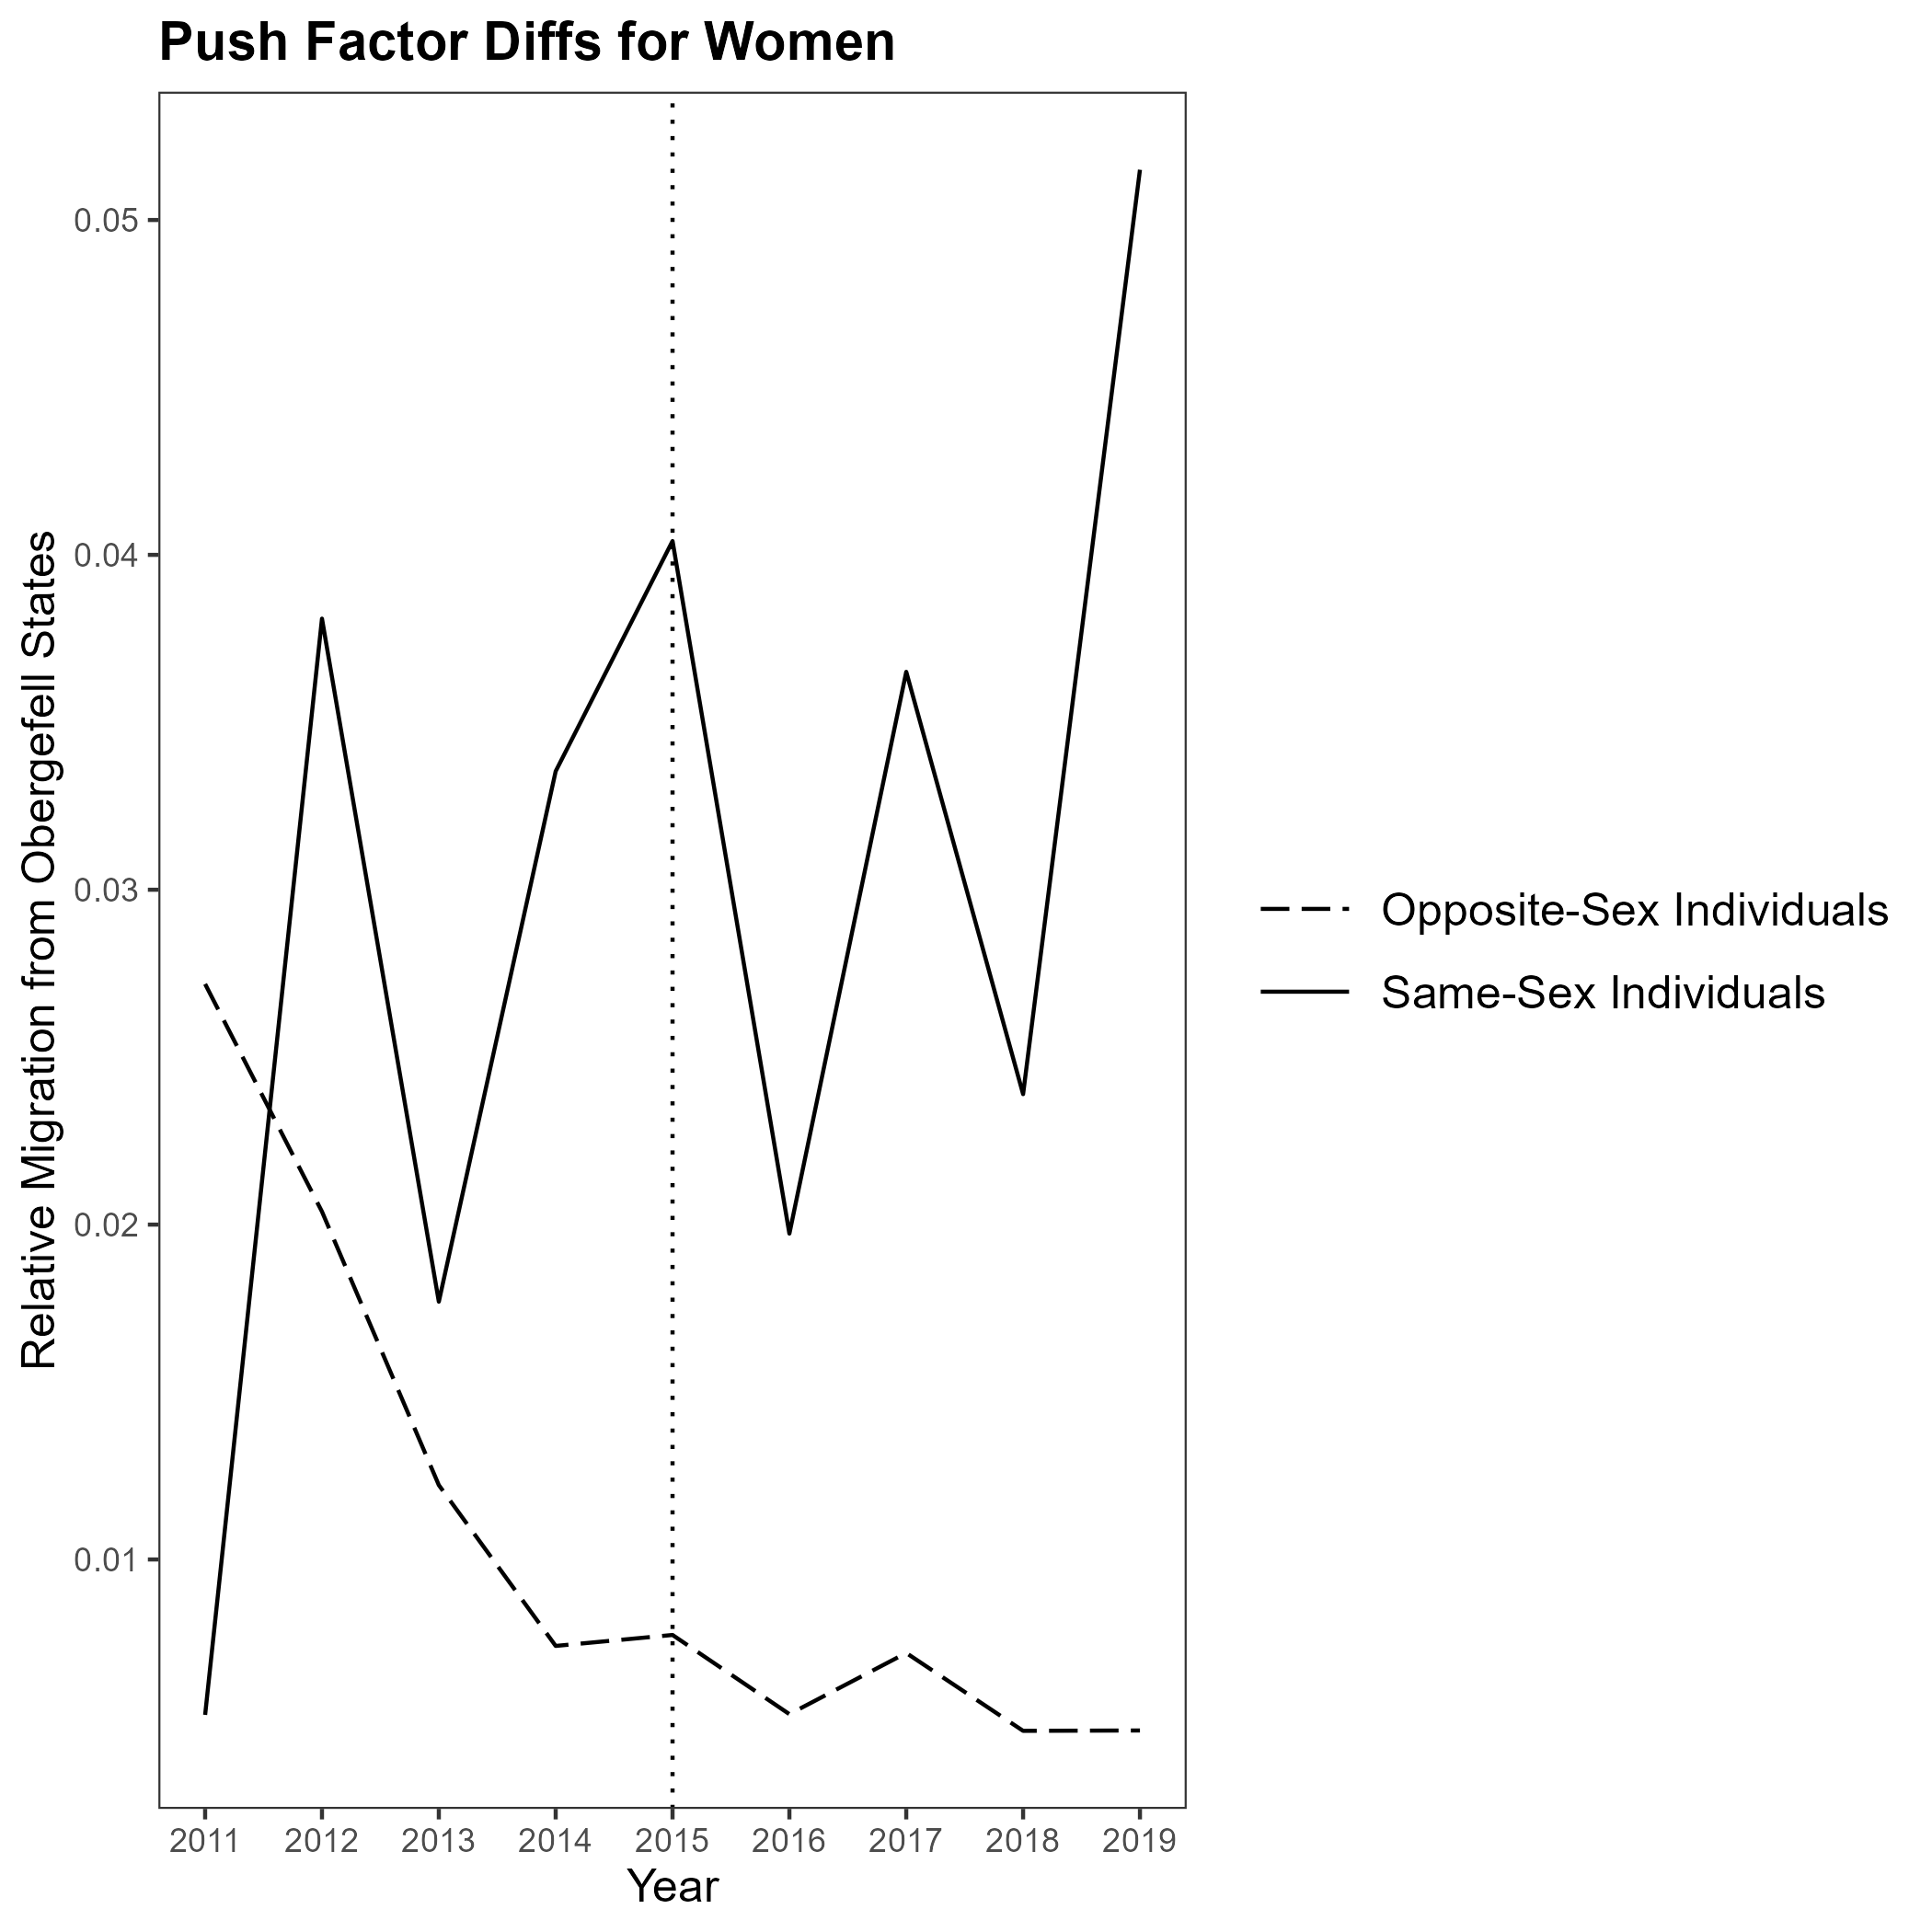
\includegraphics[width=1\linewidth]{outputs/summary_stats/sex_ante_diffs.png}
    \label{fig:enter-label}
\end{figure}

%\begin{landscape}
\centering
\tiny
\begin{tabular}{lcc}
\multicolumn{3}{c}{Ex-Ante Model} \\ \hline
 & (1) & (2) \\
VARIABLES & Model 1: Male & Model 1: Female \\ \hline
 &  &  \\
ante\_treatment & -0.005 & -0.010 \\
 & (0.010) & (0.013) \\
Constant & 0.185*** & 0.186*** \\
 & (0.000) & (0.000) \\
 &  &  \\
Observations & 481,915,892 & 474,321,020 \\
 R-squared & 0.004 & 0.004 \\ \hline
\multicolumn{3}{c}{ Robust standard errors in parentheses} \\
\multicolumn{3}{c}{ *** p$<$0.01, ** p$<$0.05, * p$<$0.1} \\
\multicolumn{3}{c}{ See below.} \\
\end{tabular}

%\end{landscape}

%\subsection{Other Heterogeneity Tests}


\subsection{Migration Flows in More Detail}
\clearpage
\begin{figure}
    \centering
    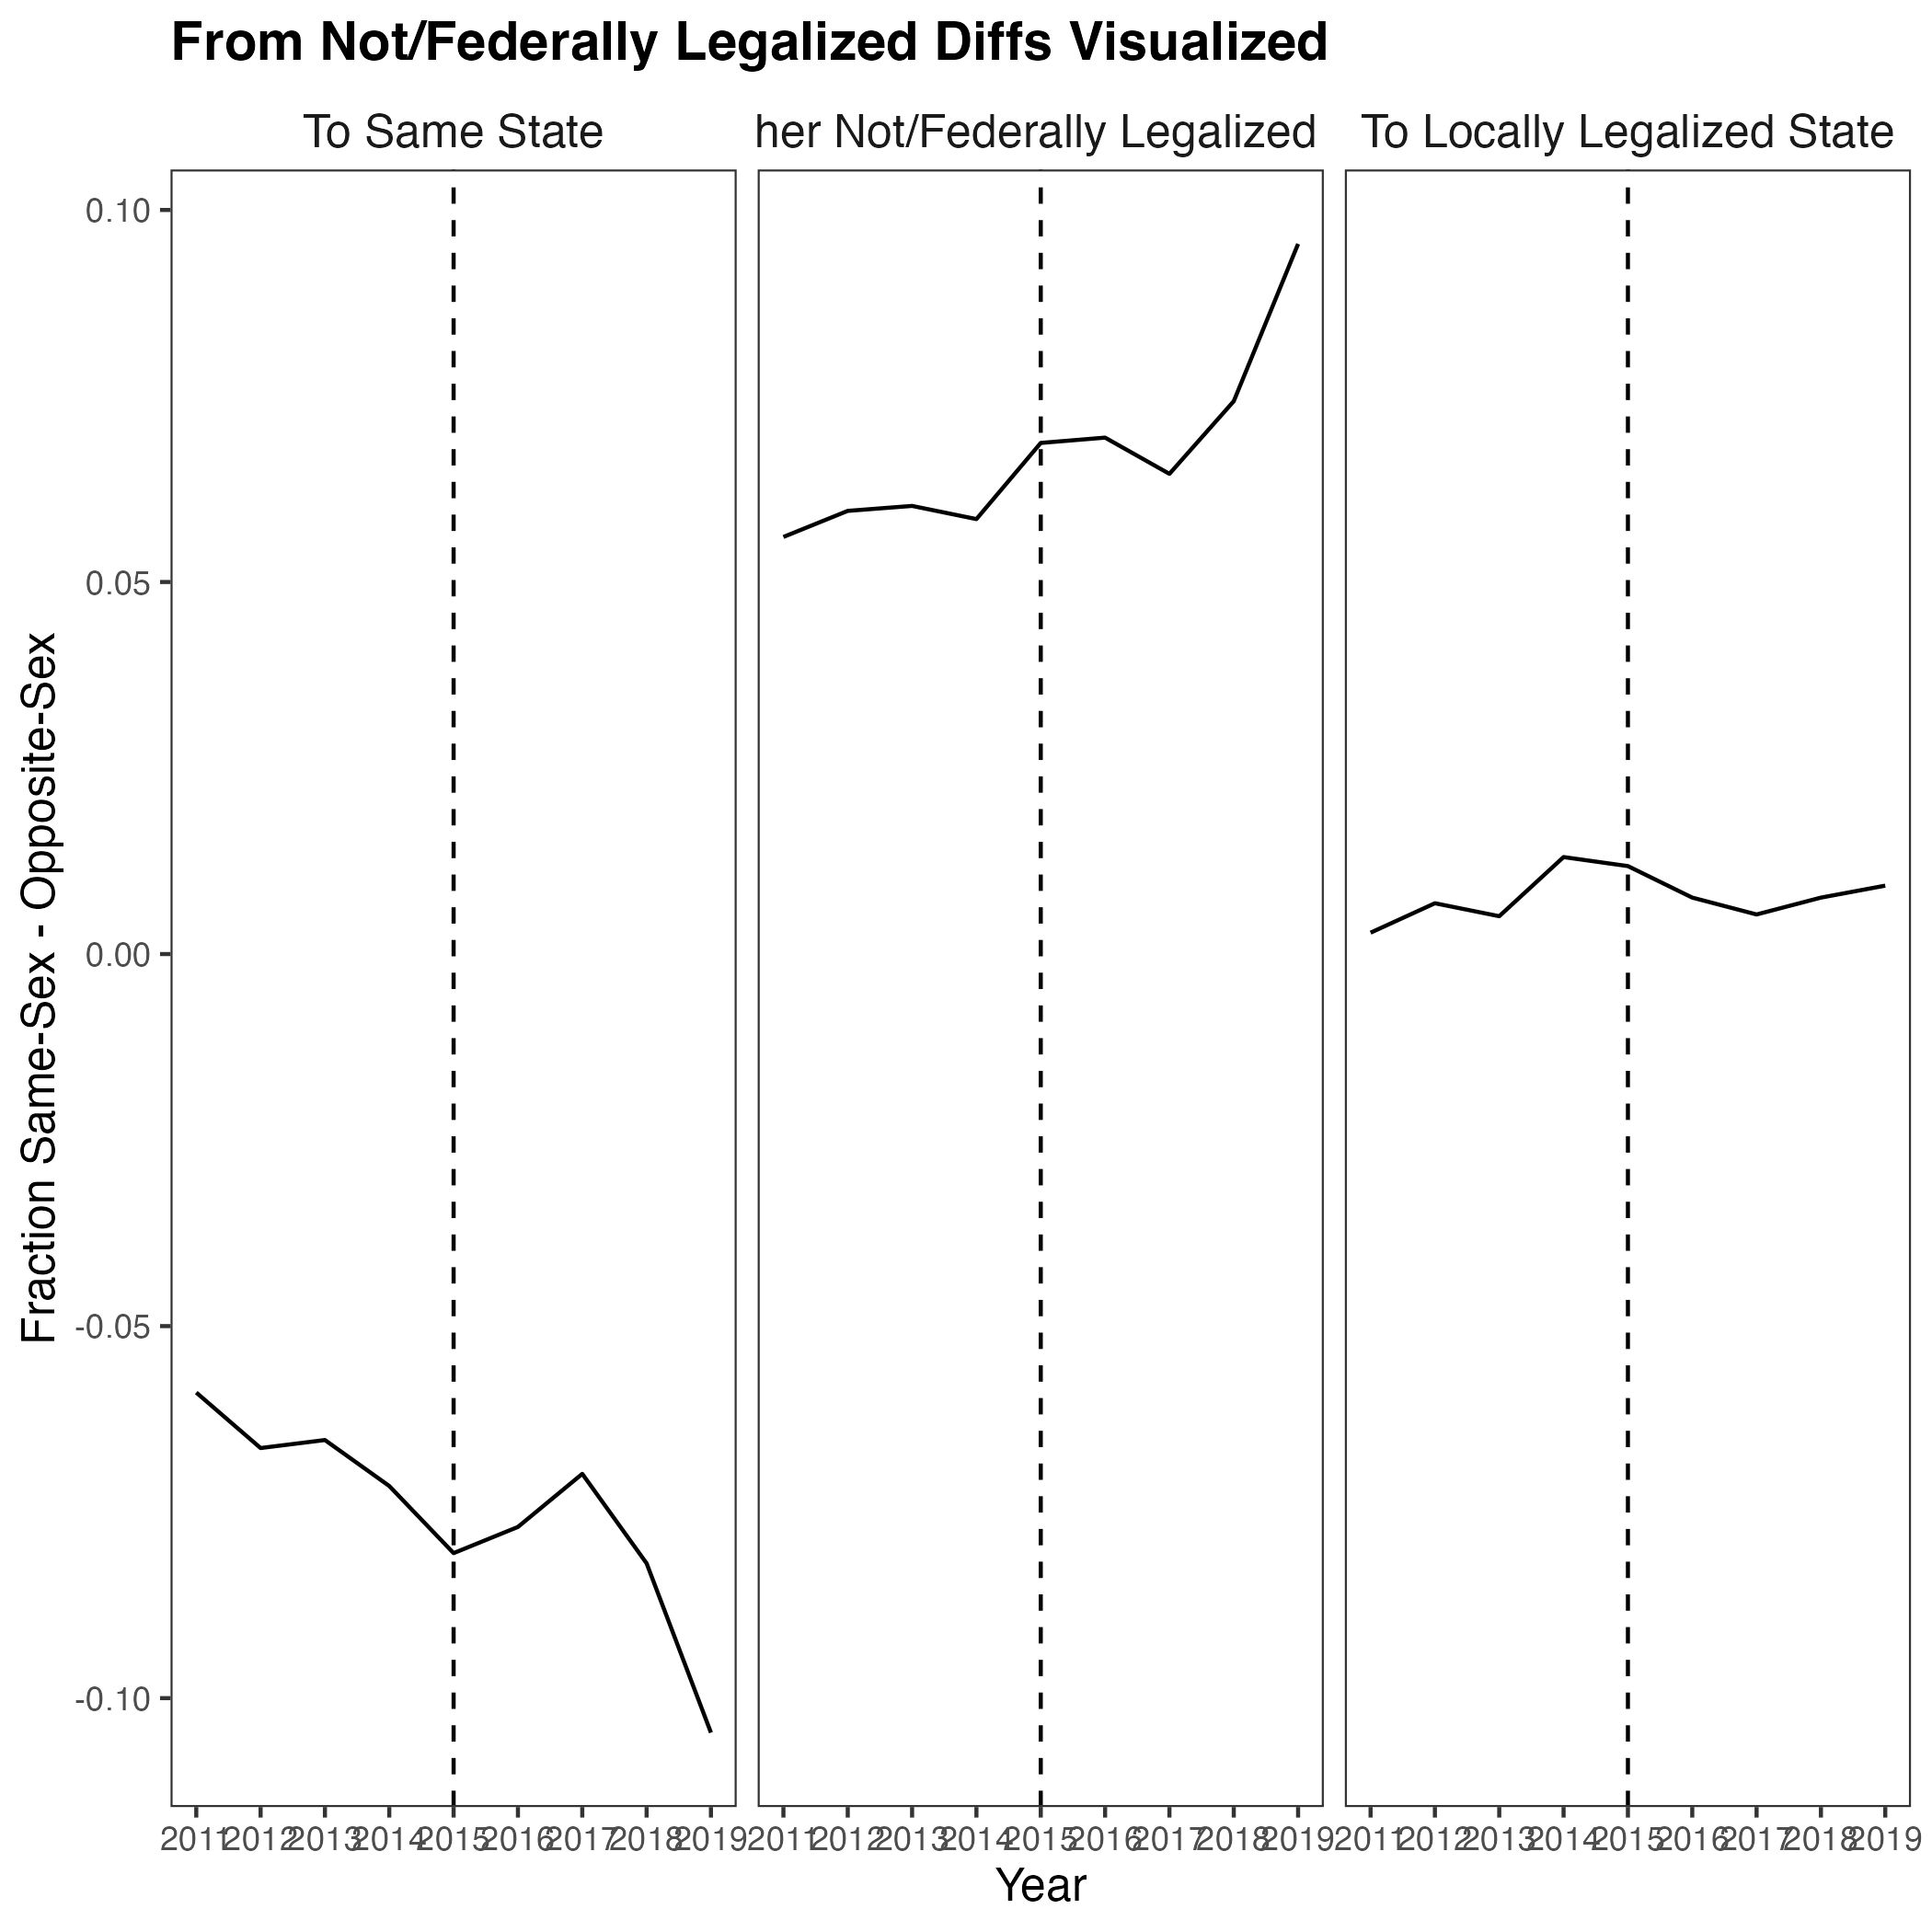
\includegraphics[width=1\linewidth]{outputs/summary_stats/from_fed_diffs.png}
    \caption{Enter Caption}
    \label{fig:enter-label}
\end{figure}

\begin{figure}
    \centering
    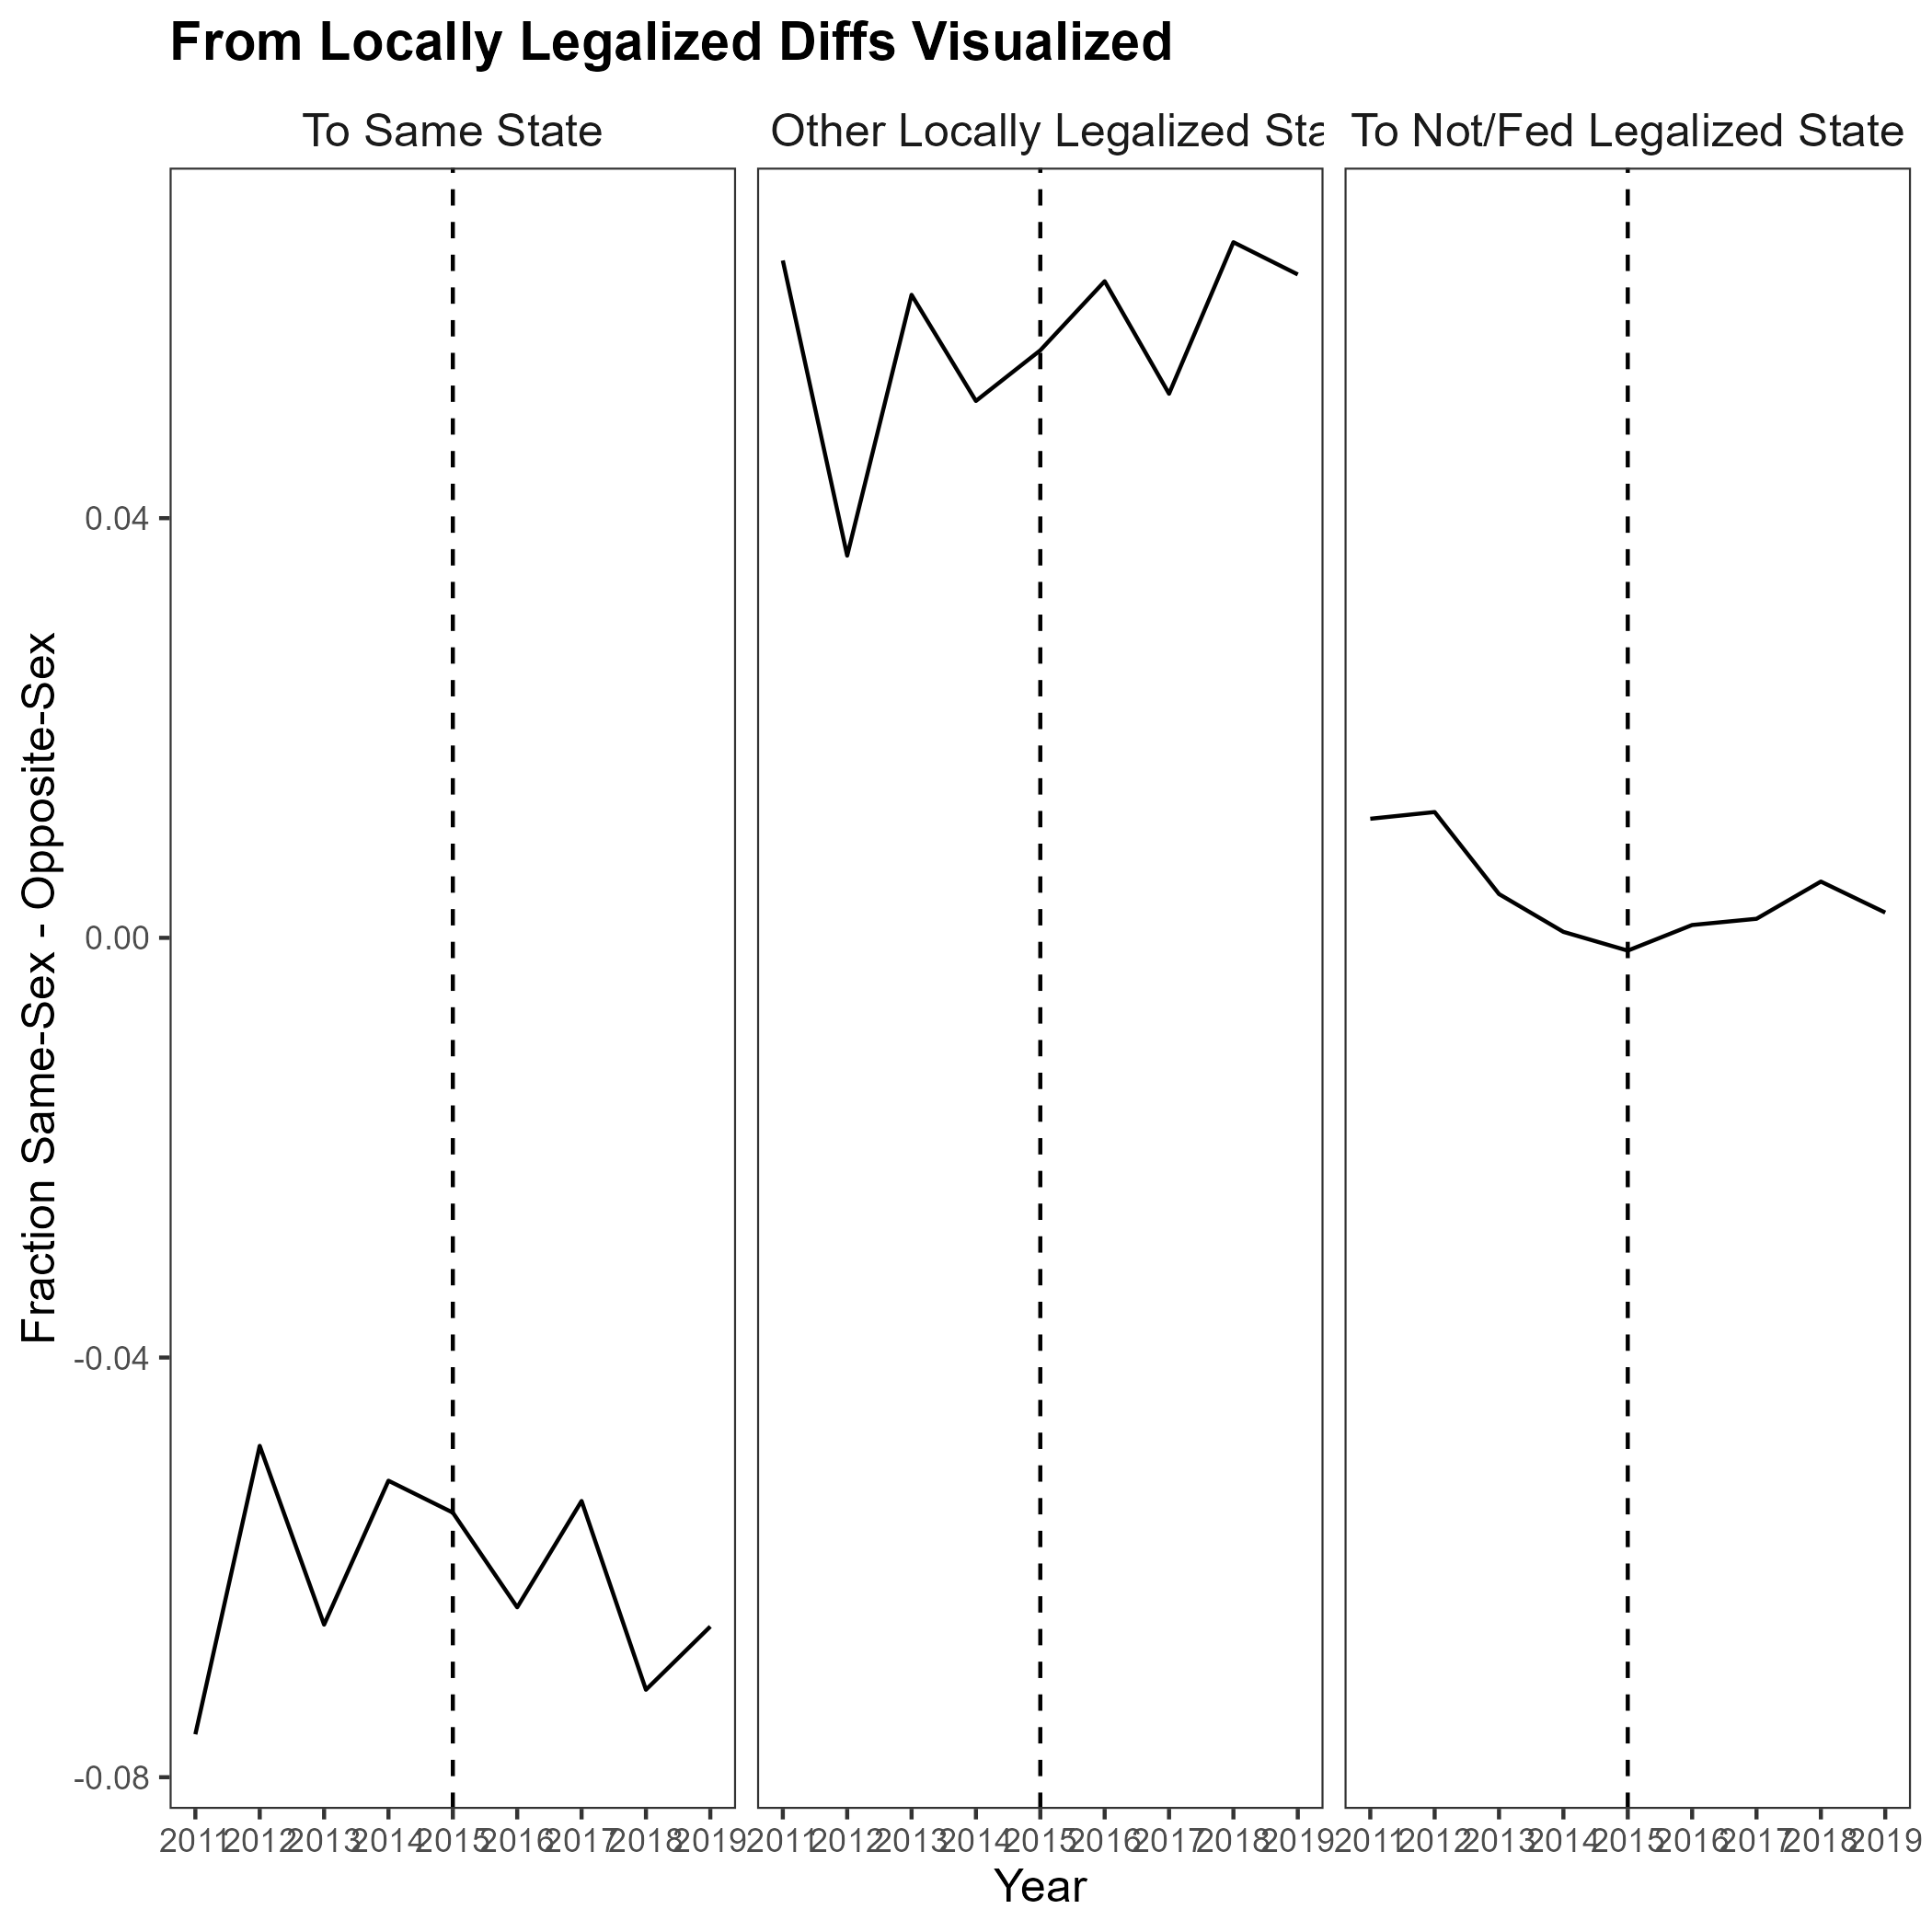
\includegraphics[width=1\linewidth]{outputs/summary_stats/from_local_diffs.png}
    \caption{Enter Caption}
    \label{fig:enter-label}
\end{figure}

\begin{tabular}{lccccccccc} \hline
 & (1) & (2) & (3) & (4) & (5) & (6) & (7) & (8) & (9) \\
VARIABLES & M1: From Fed/Not & M1: From Local & M1: Stay & M2: From Fed/Not & M2: From Local & M2: Stay & M3: From Fed/Not & M3: From Local & M3: Stay \\ \hline
 &  &  &  &  &  &  &  &  &  \\
post\_treatment & -0.035*** & 0.025** & 0.010 & -0.016 & 0.015 & 0.001 & -0.005 & 0.004 & 0.002 \\
 & (0.010) & (0.011) & (0.008) & (0.029) & (0.023) & (0.026) & (0.034) & (0.030) & (0.030) \\
Constant & 0.103*** & 0.000*** & 0.897*** & 1.968*** & 2.095*** & -3.063*** & 1.812*** & 2.102*** & -2.913*** \\
 & (0.000) & (0.000) & (0.000) & (0.325) & (0.350) & (0.131) & (0.342) & (0.352) & (0.108) \\
 &  &  &  &  &  &  &  &  &  \\
Observations & 19,755 & 19,755 & 19,755 & 19,755 & 19,755 & 19,755 & 19,755 & 19,755 & 19,755 \\
 R-squared & 0.047 & 0.046 & 0.005 & 0.531 & 0.511 & 0.922 & 0.557 & 0.548 & 0.927 \\ \hline
\multicolumn{10}{c}{ Robust standard errors in parentheses} \\
\multicolumn{10}{c}{ *** p$<$0.01, ** p$<$0.05, * p$<$0.1} \\
\multicolumn{10}{c}{ See below.} \\
\end{tabular}

\begin{tabular}{lccccccccc} \hline
 & (1) & (2) & (3) & (4) & (5) & (6) & (7) & (8) & (9) \\
VARIABLES & M1: To Fed/Not & M1: To Local & M1: Stay & M2: To Fed/Not & M2: To Local & M2: Stay & M3: To Fed/Not & M3: To Local & M3: Stay \\ \hline
 &  &  &  &  &  &  &  &  &  \\
ante\_treatment & -0.031*** & 0.023* & 0.008 & -0.011 & 0.011 & -0.000 & 0.001 & 0.002 & -0.003 \\
 & (0.008) & (0.011) & (0.012) & (0.024) & (0.022) & (0.024) & (0.027) & (0.029) & (0.025) \\
Constant & 0.181*** & 0.005*** & 0.814*** & 0.288 & 3.639*** & -2.927*** & 0.498 & 3.561*** & -3.059*** \\
 & (0.000) & (0.000) & (0.000) & (0.822) & (0.802) & (0.189) & (0.926) & (0.874) & (0.226) \\
 &  &  &  &  &  &  &  &  &  \\
Observations & 956,236,912 & 956,236,912 & 956,236,912 & 956,236,912 & 956,236,912 & 956,236,912 & 956,236,912 & 956,236,912 & 956,236,912 \\
 R-squared & 0.047 & 0.045 & 0.004 & 0.494 & 0.533 & 0.919 & 0.527 & 0.559 & 0.921 \\ \hline
\multicolumn{10}{c}{ Robust standard errors in parentheses} \\
\multicolumn{10}{c}{ *** p$<$0.01, ** p$<$0.05, * p$<$0.1} \\
\multicolumn{10}{c}{ See below.} \\
\end{tabular}


%\subsection{State Comparisons- ie something like CA v TX}

\section{Conclusion}
tbd

\newpage
% References section
\bibliographystyle{chicago}
\bibliography{Drafting/thesis_bibliography}
watch output everything even if not in text citations above
\end{document}